\section*{Kapitel 2 - Das multiple lineare Regressionsmodell}

\begin{multicols*}{3}

\tikzstyle{mybox} = [draw=black, fill=white, very thick,
    rectangle, rounded corners, inner sep=10pt, inner ysep=10pt]
\tikzstyle{fancytitle} =[fill=black, text=white, font=\bfseries]




%------------ multiple lineare Regressionsmodell ---------------
\begin{tikzpicture}
    \node [mybox] (box){%
        \begin{minipage}{0.3\textwidth}
        Das \tc{multiple lineare Regressionsmodell} hat die Form
        $$Y_i = \underbrace{\gb0 + \gb1 x_{i1} + \dots + \gb{p} x_{ip}}_{\bx_i^\top = (1, x_{i1}, \dots, x_{ip})} 
        + \eps_i; i = 1,\dots,n$$
        oder in Matrix-Vektor Notation:
        $\bY = \bX \bbeta + \beps$
        mit \\
        $ \bY = \begin{pmatrix}
            Y_1 \\ \vdots \\ Y_n
        \end{pmatrix} ,
        \bX = \begin{pmatrix}
            1 & x_{11} & \dots & x_{1p} \\
            \vdots & \vdots & \ddots & \vdots \\
            1 & x_{n1} & \dots & x_{np}
        \end{pmatrix} ,\\
        \bbeta = \begin{pmatrix}
            \gb0 \\ \vdots \\ \gb{p}
        \end{pmatrix} ,
        \beps = \begin{pmatrix}
            \eps_1\\ \vdots \\ \eps_n
        \end{pmatrix}$.\\
        Wir nehmen dabei an, dass $\bX \in \R^{n \times (p+1)}$ eine feste 
        Design-Matrix ist und dass $\beps \sim \Ncal(\bm0, \ssd \bI)$
        \end{minipage}
    };
%------------ multiple lineare Regressionsmodell Header ---------------------
\node[fill = black, text=white, font=\bfseries, right=10pt] at (box.north west) {Multiples lineares Regressionsmodell};
\end{tikzpicture}
    
%------------ KQ Schätzer ---------------
\begin{tikzpicture}
\node [mybox] (box){%
    \begin{minipage}{0.3\textwidth}
    Wir schätzen den Parameter(vektor) $\bbeta$ durch 
    \begin{align}
        \hbbeta = \argmin_{\bbeta \in \mathds{R}^{p+1}} (\bY - \bX \bbeta)^\top (\bY - \bX \bbeta)
    \end{align}
    und nennen $\hbbeta$ den \tc{KQ-Schätzer von $\bbeta$} und \\
    $\hat{\eps}_i := Y_i - \bx_i^\top \hbbeta$ die \tc{Residuen}.
    \end{minipage}
};
%------------ KQ Schätzer Header ---------------------
\node[fill = black, text=white, font=\bfseries, right=10pt] at (box.north west) 
{Kleinste Quadrate (KQ) Schätzer};
\end{tikzpicture}
    
    
%------------ Existenz und Berechnung vom KQ Schätzer ---------------
\begin{tikzpicture}
\node [mybox] (box){%
    \begin{minipage}{0.3\textwidth}
    Der KQ-Schätzer existiert und ist eindeutig, falls $\bX^\top\bX$ invertierbar ist.
    Dieser lässt sich berechnen als 
    \begin{align*}
        \hbbeta = (\bX^\top\bX)^{-1} \bX^\top \bY
    \end{align*}
    Durch differenzieren von der Gleichung (2) erhält man $\hbbeta$ als Lösung der 
    \tc{Normalengleichung}
    \begin{align*}
        \bX^\top \hbeps = 0
    \end{align*}
    \end{minipage}
};
%------------ Existenz und Berechnung vom KQ Schätzer Header --------
\node[fill = purple, text=white, font=\bfseries, right=10pt] at (box.north west) 
{Existenz und Berechnung vom KQ Schätzer};
\end{tikzpicture}

%------------ Interpretation der Modellparameter ---------------
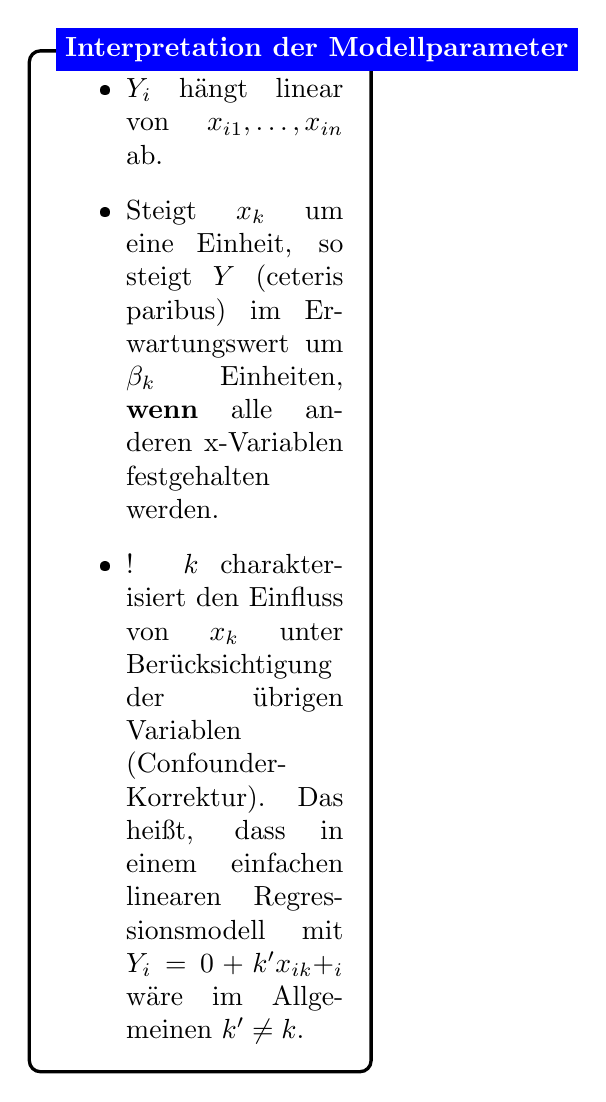
\begin{tikzpicture}
    \node [mybox] (box){%
        \begin{minipage}{0.3\textwidth}
        \begin{itemize}
            \item $Y_i$ hängt linear von $x_{i1}, \dots, x_{in}$ ab.
            \item Steigt $x_k$ um eine Einheit, so steigt $Y$ (ceteris paribus) im Erwartungswert 
            um $\beta_k$ Einheiten, \textbf{wenn} alle anderen
            x-Variablen festgehalten werden.
            \item \tc{!} $\gb{k}$ charakterisiert den Einfluss von $x_k$ 
            unter Berücksichtigung der übrigen Variablen (Confounder-Korrektur). 
            Das heißt, dass in einem einfachen linearen Regressionsmodell mit $Y_i = \gb0 + \gb{k}' x_{ik} + \eps_i$
            wäre im Allgemeinen $\gb{k}' \neq \gb{k}$.
        \end{itemize}
        \end{minipage}
    };
%------------ Interpretation der Modellparameter Header ---------------------
\node[fill = blue, text=white, font=\bfseries, right=10pt] at (box.north west) {Interpretation der Modellparameter};
\end{tikzpicture}

%------------ Eigenschaften des KQ-Schätzers ---------------
\begin{tikzpicture}
    \node [mybox] (box){%
        \begin{minipage}{0.3\textwidth}
        Gegeben dem multiplen linearen Modell, gilt für den KQ-Schätzer $\hbbeta$
        \begin{itemize}
            \item Erwartungstreue: $\E(\hbbeta) = \bbeta$. \\
            \tc{!} Gilt auch ohne die Annahme $\beps \sim \Ncal(\bm0, \ssd \bI)$, solange $\E(\beps) = \bm0$
            \item $\V(\hbbeta) = \ssd (\bX^\top\bX)^{-1}$.\\
            \tc{!} Gilt auch ohne die Annahme $\beps \sim \Ncal(\bm0, \ssd \bI)$, solange $\Cov(\beps) = \ssd \bI$
            \item $\hbbeta \sim \Ncal(\bbeta,\ssd (\bX^\top\bX)^{-1})$
        \end{itemize}
        \end{minipage}
    };
%------------ Eigenschaften des KQ-Schätzers Header ---------------------
\node[fill = purple, text=white, font=\bfseries, right=10pt] at (box.north west) {Eigenschaften des KQ-Schätzers};
\end{tikzpicture}

%------------ Hat-Matrix und Residualmatrix ---------------
\begin{tikzpicture}
    \node [mybox] (box){%
        \begin{minipage}{0.3\textwidth}
        Gegeben dem multiplen linearen Modell mit\\$\rang(\bX) = p+1$ gilt
        \begin{align*}
        \hbY := & \bX\underbrace{(\bX^\top\bX)^{-1} \bX^\top \bY}_{\hbbeta} \\
        \bP :=  & \underbrace{\bX(\bX^\top\bX)^{-1} \bX^\top}_{n \times n} \\
        \hbeps = & \bY - \hbY = (\bI - \bP)\bY\\
        \bQ := & \bI - \bP
        \end{align*}
        $\bP$ heißt \tc{Hat-Matrix} und $\bQ$ heißt \tc{Residualmatrix}.
        \end{minipage}
    };
%------------ Hat-Matrix und Residualmatrix Header ---------------------
\node[fill = black, text=white, font=\bfseries, right=10pt] at (box.north west) {Hat-Matrix und Residualmatrix};
\end{tikzpicture}

%------------ Geometrische Interpretation Hat-Matrix und Residualmatrix ---------------
\begin{tikzpicture}
    \node [mybox] (box){%
        \begin{minipage}{0.3\textwidth}
        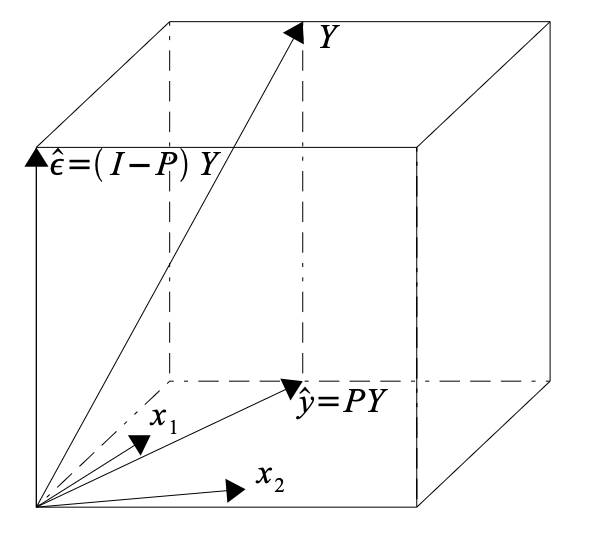
\includegraphics[scale=0.7]{fig/Projektion.png}\\
        Die KQ-Schätzung ist eine orthogonale Projektion von $\bY$ auf den von den $\bx$-Vektoren aufgespannten Unterraum.
        \end{minipage}
    };
%------------ Geometrische Interpretation Hat-Matrix und Residualmatrix Header ---------------------
\node[fill = blue, text=white, font=\bfseries, right=10pt] at (box.north west) {Geometrische Interpretation};
\end{tikzpicture}


%------------ Eigenschaften der Hat-Matrix und Residualmatrix ---------------
\begin{tikzpicture}
    \node [mybox] (box){%
        \begin{minipage}{0.3\textwidth}
        Die Hat-Matrix $\bP$ und die Residualmatrix $\bQ$ sind Projektionsmatrizen und zueinander orthogonal:
        \begin{align*}
        &\bP^\top = \bP \text{ und } \bP^2 = \bP \\
        &\bQ^\top = \bQ \text{ und }  \bQ^2 = \bQ \\
        &\bP\bQ = \bQ\bP = \bm0.
        \end{align*}
        Daraus folgt
        \begin{align*}
        &\V(\hbY) = \ssd \bP \\
        &\V(\hbeps) = \ssd \bQ, \text{ da } \hbeps = \bQ\beps
        \end{align*}
        \end{minipage}
    };
%------------ Eigenschaften der Hat-Matrix und Residualmatrix Header ---------------------
\node[fill = purple, text=white, font=\bfseries, right=10pt] at (box.north west) {Eigenschaften von $\bP$ und $\bQ$};
\end{tikzpicture}


%------------ Schätzer für $\ssd$ ---------------
\begin{tikzpicture}
    \node [mybox] (box){%
        \begin{minipage}{0.3\textwidth}
        Gegeben dem multiplen linearen Modell, gilt
        $$\hat{\sd}^2 := \frac{\hbeps^\top\hbeps}{n-(p+1)} = \frac{1}{n-(p+1)} \sumin \hat{\eps}_i^2$$ 
        ist ein erwartungstreuer Schätzer von $\ssd$.\\
        \tc{!} Gilt auch ohne die Annahme $\beps \sim \Ncal(\bm0, \ssd \bI)$, solange $\E(\beps) = \bm0$ und $\Cov(\beps) = \ssd \bI$
        \end{minipage}
    };
%------------ Schätzer für $\ssd$ Header ---------------------
\node[fill = purple, text=white, font=\bfseries, right=10pt] at (box.north west) {Schätzer für $\ssd$};
\end{tikzpicture}
    


%------------ Überschrift ---------------

\begin{tikzpicture}
    \node [mybox] (box){%
        \begin{minipage}{0.3\textwidth}
        
        \end{minipage}
    };
%------------ Überschrifts Header ---------------------
\node[fill = black, text=white, font=\bfseries, right=10pt] at (box.north west) {Überschrift};
\end{tikzpicture}
    
\end{multicols*}